\documentclass[main]{subfiles}
\begin{document}

\section*{Lecture 9 // Sept 22 // Singularities in $\mc{M}$, part 2}
\addcontentsline{toc}{section}{Lecture 9 -- Singularities in M, part 2}

\begin{recall}
We saw that connections whose stabilizer is larger than $\pm\mathrm{Id}$ lead to singular points of $\mc{M}$, and this does happen.

If $E$ is split and $\nabla$ is split, then $\Stab(\nabla)$ is at least as large as $S^1$. Precisely, we had the following lemma:
\[
\text{If } E \text{ is a } k\neq 0\ \SU(2) \text{ bundle, then } \Stab(\nabla) \text{ is larger than } \pm I
\]
\[
\text{iff } \nabla \text{ is split, in which case } \Stab(\nabla)\cong S^1.
\]
Towards proving this lemma, we discussed parallel transport and holonomy.
\end{recall}

The general question is what are the possibilities of $\Stab(\nabla)$? A priori, we know that $\Stab(\nabla)\subseteq \mc{G}$, and this fact actually restricts what $\Stab(\nabla)$ must be as follows.

\begin{lemma}
$g\in\Stab(\nabla)$ iff $D_\nabla g = 0$, where $D_\nabla : \End(E)\to \End(T^\ast M\otimes E)$, i.e., $g$ is parallel transported by $D_\nabla$ along every $\gamma$.
\end{lemma}

\begin{proof}
$D_\nabla g$ is characterized by the Leibniz rule:
\[
\nabla(gs) = (D_\nabla g)s + g(\nabla s)
\]
After moving terms, we get
\[
g^{-1}\nabla(gs) = g^{-1}(D_\nabla g)s + \nabla s
\]
By definition, $g^\ast(\nabla)s = g^{-1}\nabla(gs)$.

Thus
\[
g\in\Stab(\nabla) \text{ iff } g^\ast(\nabla)=\nabla
\]
\[
\Leftrightarrow \nabla(s) = g^{-1}(D_\nabla g)s + \nabla s \quad \forall s
\]
\[
\Leftrightarrow g^{-1}(D_\nabla g)s = 0 \quad \forall s
\]
\[
\Leftrightarrow D_\nabla g = 0 \qedhere
\]
\end{proof}

Moreover, we know that the parallel transport is unique. So we can also conclude the following.

\begin{lemma}
If $g\in\Stab(\nabla)$, then $g$ is determined by its value at a single point.
\end{lemma}

\begin{remark}
It's not true that any $g$ can be transported: $g$ need not be globally defined! But we know $g\in\Stab(\nabla)$, so a priori, it \underline{is} a global object, so parallel transport makes sense.
\end{remark}

Equivalently, we can write this as for any $p$, the restriction map $\mc{G}\to\Aut(E_p)$ is injective on $\Stab(\nabla)$,
\[
g \longmapsto g_p.
\]

Thus (via restriction) $\Stab(\nabla)$ can be considered as a subgroup of $\SU(2)$. In fact, $\Stab(\nabla)$ has a nice connection with the holonomy of $\nabla$.

Recall that for a fixed $p\in M$, the holonomy gives a map
\[
\hol_p : \left\{\text{loops based at } p\right\} \longrightarrow \Aut(E_p) = \SU(2)
\]
\[
\gamma \longmapsto \hol_p^\nabla(\gamma)
\]
Very explicitly, under $\hol_p$, each $\gamma$ gets sent to a specific linear transformation $E_p$ to $E_p$, e.g., a matrix transformation of the fibre, e.g., an element of $\SU(2)$. If $\gamma$ is varied to another $\gamma'$, we get another matrix transformation.

By considering every $\gamma'$, the set of corresponding matrices is $\operatorname{im}(\hol_p)$, and since $\hol_p(\gamma_2\circ\gamma_1) = \hol_p(\gamma_2)\circ\hol_p(\gamma_1)$, $\operatorname{im}(\hol_p)$ forms a subgroup of $\SU(2)$.

\begin{lemma}
The restriction of $\Stab(\nabla)$ to a point $p$ is the centralizer of $\operatorname{im}\hol_p$.
\end{lemma}

\begin{proof}
$(\subseteq)$: Take $g\in\Stab(\nabla)$. We want to show that $g_p$ commutes with $\hol_p(\gamma)$ for every loop $\gamma$. We know that $\hol_p^{g^\ast(\nabla)}(\gamma) = g_p^{-1}\circ\hol_p^\nabla(\gamma)\circ g_p$.

Since $g\in\Stab(\nabla)$, we know $g^\ast(\nabla)=\nabla$, so $\hol_p^{g^\ast(\nabla)}(\gamma) = \hol_p^\nabla(\gamma)$.

Thus $\hol_p^\nabla(\gamma) = g_p^{-1}\circ\hol_p^\nabla(\gamma)\circ g_p$ as desired. $\square$

$(\supseteq)$: Take $g_p\in\Aut(E_p)$. Further assume that $g_p\in Z(\operatorname{im}(\hol_p))$.

We want to show that there exists some $g\in\Stab(\nabla)$ such that the restriction of $g$ to $E_p$ is $g_p$.

Since $\Stab(\nabla) = \{g \mid D_\nabla g = 0\}$, to define $g$, we should try to extend $g_p$ via parallel transport by $D_\nabla$.

For any other point $q$, let $\gamma$ be a path from $p$ to $q$.
\begin{center}
\begin{minipage}[t]{0.38\textwidth}
\centering
\vspace{0pt}
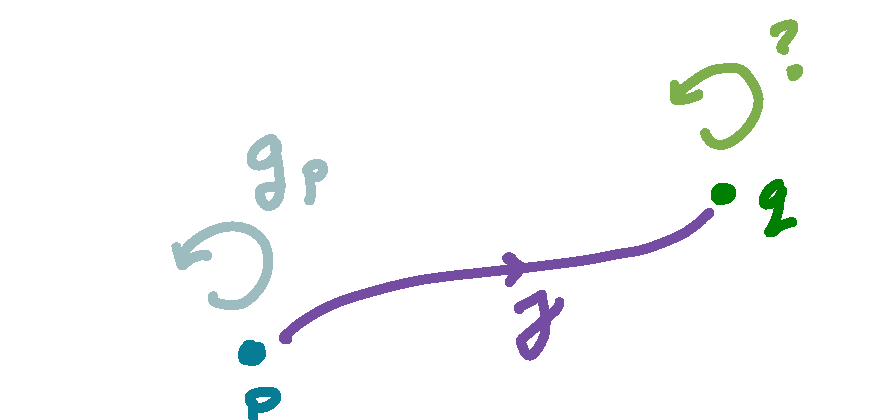
\includegraphics[width=\linewidth]{figures/fig_lec9_parallel1.png}
\end{minipage}%
\hfill
\begin{minipage}[t]{0.55\textwidth}
\vspace{0pt}
Define $g_\gamma$ such that
\begin{enumerate}
	\item[\textcircled{1}] $g_p$ is extended along $\gamma$ such that $(D_\nabla)_\gamma g = 0$
	\item[\textcircled{2}] $g_q = \hol_{p,q}(\nabla)\circ g_p \circ \hol_{q,p}(\bar\gamma)$
\end{enumerate}
\end{minipage}
\end{center}

We can do this along $\gamma$ since parallel transport exists. For any path, we can cook up a $g_\gamma$ such that $D_\nabla(g_\gamma)$ vanishes along $\gamma$; this follows by existence of solutions to ODEs.

However a priori, we don't know that this extension along $\gamma$ gives a well-defined global $g$. Take $\gamma'$ another path from $p$ to $q$, and consider $g'$ defined by $\gamma'$.

\begin{center}
\begin{minipage}[t]{0.38\textwidth}
\centering
\vspace{0pt}
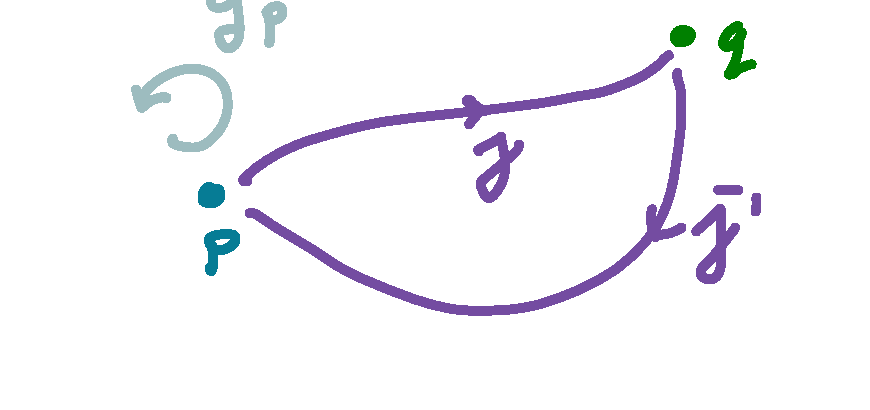
\includegraphics[width=\linewidth]{figures/fig_lec9_parallel2.png}
\end{minipage}%
\hfill
\begin{minipage}[t]{0.55\textwidth}
\vspace{0pt}
Then $g_q$ and $g'_q$ are defined as
\[
g_q = \hol(\gamma)\circ g_p \circ \hol(\bar\gamma)
\]
\[
g'_q = \hol(\gamma')\circ g_p \circ \hol(\bar\gamma').
\]
\end{minipage}
\end{center}

If $g_q$ is well defined, $g_q^{-1} = (g'_q)^{-1}$ for any other $g'_q$, i.e.,
\[
g_q(g'_q)^{-1} = \mathrm{id}.
\]
Indeed,
\[
g_q(g'_q)^{-1} = \hol(\gamma)\circ g_p\circ\hol(\bar\gamma)\,\big(\hol(\gamma')\circ g_p\circ\hol(\bar\gamma')\big)^{-1} = \mathrm{id} \qedhere
\]
\end{proof}

Let's take stock so far: we know that $\Stab(\nabla)$ is determined by its restriction to a point, which is the centralizer of the holonomy at that point, viewed as a subgroup of $\SU(2)$.

So our question now becomes what are the subgroups of $\SU(2)$?

\begin{fact}
They are as follows:
\begin{center}
\begin{tabular}{c|c}
Subgroups of $\SU(2)$ & Centralizer $=\Stab(\nabla)$ \\
\hline
$I$ & $\SU(2)$ \\
$-I$ & $\SU(2)$ \\
$S^1$ or a conjugate of $S^1$ & $S^1$ \\
Subgroups of $S^1$ or conjugate & $S^1$ \\
Non-abelian & $\pm I$ \\
$\SU(2)$ & $\pm I$
\end{tabular}
\end{center}
\end{fact}

This means that the only possibilities for $\Stab(\nabla)$ are $\pm\mathrm{Id}$, $S^1$, or $\SU(2)$ itself. We are now in the position to prove the lemma.

\begin{lemma}
If $E$ is a $k\neq 0$ $\SU(2)$ bundle, then $\Stab(\nabla)$ is larger than $\pm I$ iff $\nabla$ is split, in which case $\Stab(\nabla)\cong S^1$.
\end{lemma}

\begin{proof}
We first show that either $\Stab(\nabla)\cong S^1$ or $\pm\mathrm{Id}$. From there, we'll show the former happens iff $\nabla$ is split.

We just saw that there are only three possibilities for $\Stab(\nabla)$, so we need only to rule out $\SU(2)$.

If $\nabla$ is a connection on an $k\neq 0$ bundle, then $F_\nabla$ cannot be identically $0$ (if it was, $c_2=k=0$).

Thus holonomy can't be nontrivial, since the holonomy picks up curvature enclosed by a loop. If this path is varied, $\hol$ will vary continuously, so $\operatorname{im}(\hol_p)$ can't be contained in a discrete subgroup. Thus the centralizer cannot be $\pm I$, so the subgroup can't be $\SU(2)$.

Now, suppose $\Stab(\nabla)=S^1$. We just saw that $\Stab(\nabla)=S^1$ implies that at a point $p\in M$, the element $g_p\in\SU(2)$ must actually be contained in $U(1)\subset\SU(2)$.

Therefore
\[
g_p = \begin{pmatrix} e^{i\theta} & 0 \\ 0 & e^{-i\theta}\end{pmatrix},
\]
which induces a splitting of the fibre over $p$ by considering the eigenspaces.

For any other $q\in M$, $g_q$ is obtained from $g_p$ via conjugation with $\hol_{p,q}(\gamma)$, so the eigenspaces of $g_q$ provide a splitting of $E_q$ compatible with that of $E_p$. Since $\Stab(\nabla)$ is reconstructed from $g_p$ by parallel transport, the splitting of $E_p$ induces a splitting of $E$.

To Do: Insert proof of other direction. $\qedsymbol$
\end{proof}

Having proved this lemma, we can conclude our discussion of why the number of singular points in $\mc{M}$ is the number of splittings of $E$.

We'll now begin a discussion of the other major qualitative feature $\mc{M}$: that $\partial\bar{\mc{M}} = M$. To do so, we'll first discuss instantons ((A)SD Yang-Mills connections) on $S^4$, which we'll do by identifying $S^4$ with $\HP^1$.

\subsection*{Interlude: Review of Quaternions \& Some Useful Isomorphisms from Algebra}

\begin{definition}
A quaternion is an expression of the form $q=x+yi+zj+wk$ where $x,y,z,w\in\RR$ and $1,i,j,k$ are basis elements such that
\[
1\cdot\alpha = \alpha \text{ for } \alpha=i,j,k, \qquad i^2=j^2=k^2=ijk=-1
\]
\[
i\cdot j = k,\quad j\cdot k = i,\quad k\cdot i = j, \qquad \text{and} \qquad \alpha\cdot x = x\cdot\alpha \text{ for } \alpha=i,j,k \text{ and } x\in\RR.
\]
The space of quaternions is denoted $\HH$.
\end{definition}

\begin{remark}
$\HH$ admits the structure of a division ring. However, multiplication fails to be commutative, so $\HH$ is not a field: if $q_1=i$ and $q_2=j$, $q_1q_2 = ij \neq ji = q_2q_1$.
\end{remark}

Note that $\HH\cong\CC^2\cong\RR^4$ by the following isomorphisms. First rewrite a quaternion as
\[
x+yi+zj+wk = (x+yi)+(zj+wk) = (x+yi)+(zj+wij) = (x+yi)+(z+wi)j.
\]
Then the isomorphisms are given by the maps
\[
\HH \longrightarrow \CC^2 \longrightarrow \RR^4
\]
\[
(x+iy)+(z+iw)j \longmapsto (x+iy,\,z+iw) \longmapsto (x,y,z,w).
\]

The quaternions can also be identified by a specific subgroup of the space of $2\times 2$ complex matrices.

\begin{definition}
The Pauli matrices are a set of three $2\times 2$ matrices $\{\sigma_1,\sigma_2,\sigma_3\}\subset \Mat_{2\times 2}(\CC)$ which are traceless, Hermitian, unitary, and involutive:
\[
\sigma_1 := \begin{pmatrix} i & 0 \\ 0 & -i\end{pmatrix} \qquad \sigma_2 := \begin{pmatrix} 0 & 1 \\ -1 & 0\end{pmatrix} \qquad \sigma_3 := \begin{pmatrix} 0 & i \\ i & 0\end{pmatrix}
\]
\end{definition}

By sending $i\mapsto\sigma_1$, $j\mapsto\sigma_2$, and $k\mapsto\sigma_3$, any quaternion $q=x+yi+zj+wk$ can be rewritten as the linear combination
\[
x\,\mathrm{Id}+y\sigma_1+z\sigma_2+w\sigma_3 = \begin{pmatrix} x & 0 \\ 0 & x\end{pmatrix} + \begin{pmatrix} yi & 0 \\ 0 & -yi\end{pmatrix} + \begin{pmatrix} 0 & z \\ -z & 0\end{pmatrix} + \begin{pmatrix} 0 & wi \\ wi & 0\end{pmatrix}
\]
\[
= \begin{pmatrix} x+yi & z+wi \\ -z+wi & x-yi\end{pmatrix}.
\]

Now, notice that the $(2,2)$ entry is the complex conjugate of the $(1,1)$ entry, and the $(2,1)$ entry is the negative conjugate of the $(1,2)$ entry. This relationship is clearly from the chosen basis vectors, so it holds for the image of any quaternion:
\[
q \longmapsto \begin{pmatrix} \alpha & \beta \\ -\bar\beta & \bar\alpha\end{pmatrix} \qquad \text{where} \qquad q = \alpha+\beta j.
\]

By now, matrices of this form should be familiar. If we divide by the norm, we recover the $\SU(2)$ matrices!

\begin{proposition}
The Lie group $\SU(2) = \left\{\begin{pmatrix}\alpha & -\bar\beta \\ \beta & \bar\alpha\end{pmatrix} \ \middle|\ \alpha,\beta\in\CC,\ |\alpha|^2+|\beta|^2=1\right\}$ is isomorphic (as a ring) to the ring of unit quaternions.
\end{proposition}

Recall that $\SU(2)$ is the $2\times 2$ complex matrices of determinant one. By identifying $\CC^2$ with $\RR^4$, an element of $\SU(2)$ determines a determinant one $4\times 4$ matrix, i.e., a rotation in $\RR^4$. Rotations in $\RR^4$ are determined by a rotation of the unit sphere $S^3\subset\RR^4$, which is determined by the image of the $(1,0,0,0)$ vector, which is a point on $S^3$. This suggests the following claim.

\begin{proposition}
$\SU(2)$ is diffeomorphic to $S^3$.
\end{proposition}

\begin{exercise}
Prove this proposition.
\end{exercise}

All together, we can conclude that $\SU(2) \cong \{q\in\HH \mid |q|^2=1\} \cong S^3$.

We can now ask: what is $\HP^1$? We now have the tools to understand why $\HP^1\cong S^4$.

Recall that one construction of the projective spaces $\RR P^1$ and $\CC P^1$ are as the one point compactifications of $\RR$ and $\CC$, respectively; since $\HH\cong\RR^4$ and $\RR^4\cup\{\infty\}\cong S^4$, we can conclude that $\HP^1\cong S^4$!

Alternatively, recall that $\RR P^n$ is most commonly constructed as the quotient of $S^n$ by the antipodal map. By viewing the antipodal map as the action of the ``unit circle'' $\{\pm 1\}\subset\RR$, and further identifying $\{\pm 1\}\cong S^0$, $\RR P^n$ can be seen as the base space of a fibration $p : S^n\to\RR P^n$ with $S^0$ fibres. This construction is easily generalized to $\CC P^n$ and then $\HP^n$: let $V$ be a vector space over the ring $k=\RR,\CC,$ or $\HH$, and let $U(V^d)$ be the unit circle in $V^d$.

When $k=\RR$, $V^{n+1}$ is $n+1$ real dimensions, so $U(V_\RR^{n+1})\cong S^{n+1-1}=S^n$. The unit circle in $\RR$ is $\{\pm 1\}\cong S^0$. This recovers the fibration
\[
S^0 \to S^n \to \RR P^n.
\]

When $k=\CC$, $V^{n+1}$ is $2(n+1)$ real dimensions, so $U(V_\CC^{n+1})\cong S^{2(n+1)-1}=S^{2n+1}$. The unit circle in $\CC\cong\RR^2$ is $\{e^{i\theta}\}\cong S^1$, so the fibration becomes
\[
S^1 \to S^{2n+1} \to \CC P^n.
\]
Note that when $n=1$, this recovers the standard Hopf fibration $S^1\to S^3\to S^2$.

When $k\cong\HH$, $V^{n+1}$ is $4(n+1)$ real dimensions, so $U(V_\HH^{n+1})\cong S^{4(n+1)-1}=S^{4n+3}$. The unit circle in $\HH\cong\RR^4$ is $S^3$, thus the fibration is
\[
S^3 \to S^{4n+3} \to \HP^n.
\]

\subsection*{Instantons on $S^4$}

Mirroring our previous discussion of instantons on $\CC P^1$, we'll view $S^4=\HP^1$. $\HP^1$ admits two charts $U_0,U_1\cong\RR^4\cong\HH$, with the coordinate change function given by $q\mapsto \frac1q$.

\begin{wrapfigure}{r}{0.38\textwidth}
\centering
\vspace{-1em}
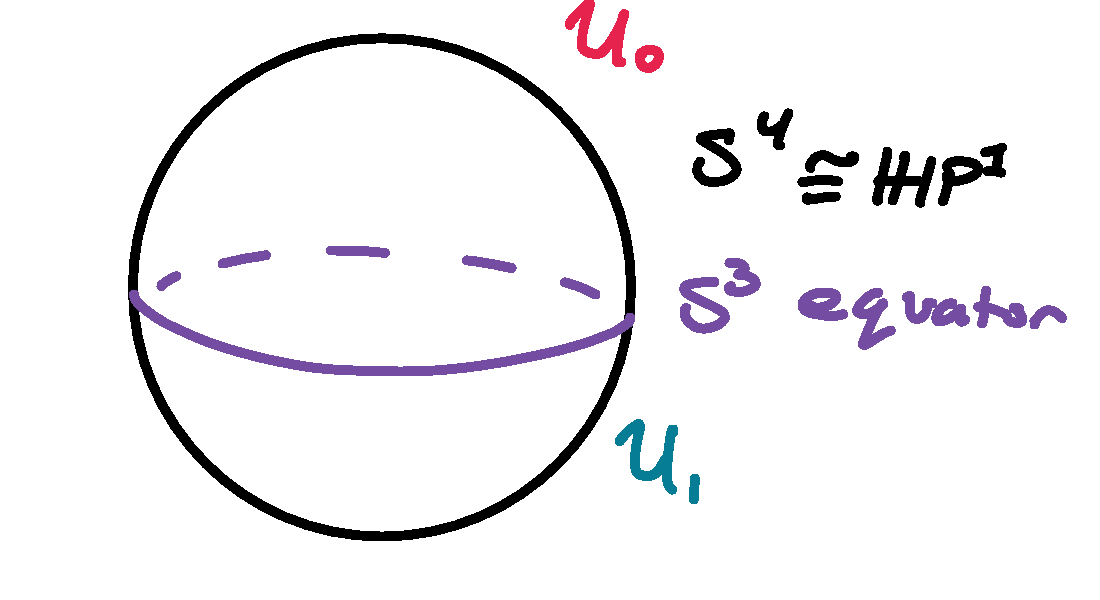
\includegraphics[width=\linewidth]{figures/fig_lec9_hp1.png}
\end{wrapfigure}
What are $\SU(2)$ bundles over $S^4$?

$\SU(2)$ bundles correspond to maps $S^3\to\SU(2)$, where $S^3$ is the region on which we glue $U_0$ to $U_1$. Since $\SU(2)\cong S^3$, $\SU(2)$ bundles over $S^4$ are classified by maps $S^3\to S^3$, of which there are $\ZZ$-many (degree).

In terms of coordinates, some possible gluing maps are $g(q) = q^n/|q|^n$.

The $k=1$ bundle corresponds to $g(q)=q$.

\end{document}
